% Example use of document class for research/technical/research review reports
% at CTU FIT (http://fit.cvut.cz)
% 2015/04/12 Created by Ondrej Guth <ondrej.guth@fit.cvut.cz>



% Nutno napsat v souladu s metodickym pokynem pro vydavani 
% vyzkumnych, souhrnnych a technickych zprav na FIT CVUT




% % % % 
% OPTIONS of the class
% LANGUAGE:
% czech 
% english
% TYPE
% research
% technical
% review
% FONT NORMALSIZE
% 10pt
% 11pt
% 12pt
% % 
\documentclass[english,technical,10pt]{FITreport}[2018/01/26]

\usepackage[utf8]{inputenc}

\usepackage{lmodern} % unicode version of Computer Modern font
\usepackage{amsthm}
% \usepackage{hyperref}

% % % % % 
% Use ALL of the following commands
% % % % % 

\title{The State-of-the-Art of Automated Testing of Models of Cyber-Physical Systems\thanks{The research has been supported by SGS grant No. SGS17/213/OHK3/3T/18}}
\author{Tomáš Apeltauer\thanks{The author would like to express his gratitude for intellectual support, ideas and feedback, to his supervisor doc. Dipl.-Ing. Dr. techn. Stefan Ratschan.}\affil{Department of Digital Design\\\theFIT}
	}
\abstractL{Abstract in language of this report.}
\abstractEN{Abstract in English (used only with reports written in Czech).}
\keywordsL{list of keywords in language of this report}
\keywordsEN{list of keywords in English (used only with reports written in Czech).}
\reportNumber{02}
\reportYear{18}
\published{January 2018}

% % % % % % % % % % 

\begin{document}

\theoremstyle{definition}
\newtheorem{lemma}{Lemma}
\newtheorem{theorem}[lemma]{Theorem}
\newtheorem{definition}[lemma]{Definition}
\newtheorem{preposition}[lemma]{Preposition}
\newtheorem{example}[lemma]{Example}
\newtheorem{corollary}[lemma]{Corollary}
\newtheorem{proposition}[lemma]{Proposition}
\newtheorem{property}[lemma]{Property}
\newtheorem{observation}[lemma]{Observation}
\theoremstyle{remark}
\newtheorem{notation}[lemma]{Notation}
\newtheorem{note}[lemma]{Note}




\section{Introduction}

Here will go some intro talk...

\subsection{Some subsection}


\section{Cyber-physical systems}

The concept of a cyber-physical system is a generalization of embedded systems. An embedded system consists of hardware and software integrated within a mechanical or and electrical system designed for a specific purpose. The term Cyber-Physical Systems is a buzzword  nowadays and it is not easy to define it. Take these three definitions from different academic sources.

\begin{definition}[Cyber-Physical Systems]
    Represents transformative technologies for managing interconnected systems between its physical assets and computational capabilities. [A Cyber-Physical Systems architecture for Industry 4.0-based manufacturing systems Jay Lee, Behrad Bagheri, Hung-An Kao]
\end{definition}

\begin{definition}[Cyber-Physical Systems]
    Refers to a new generation of systems with integrated computational and physical capabilities that can interact with humans through many new modalities. [The Impact of Control Technology Published by: IEEE Control Systems Society February 2011 Radhakisan Baheti and Helen Gill]

\end{definition}

\begin{definition}[Cyber-Physical Systems]
    Are physical and engineered systems whose operations are monitored, coordinated, controlled and integrated by a computing and communication core.[Cyber-Physical Systems: The Next Computing Revolution, Lee , Sha, Stankovic]

\end{definition}

\begin{definition}\label{def:Rajeev}[Cyber-Physical Systems]
    Consist of a collection of computing devices communicating with one another and interacting with the physical world via sensors and actuators in a feedback loop. [Rajeev, Principles of Cyber-physical systems]
\end{definition}

In this paper, we will be assuming Definition~\ref{def:Rajeev}. Cyber-Physical Systems (CPS) consist of a computational unit, sensors, actuators and a physical world which it must observe and react on it. CPS are reactive systems which interacts with its environment in an ongoing manner. There is an endless loop of data collection and input evaluation throughout the time. In a cyber-physical system, the controller consists of discrete software concurrent components operating in multiple modes of operation, interacting with the continuously evolving physical environment.

\subsection{Motivation for using Cyber-Physical Systems}

Advance in the field of Cyber-physical systems will bring us closer to usage of high-speed, low-cost, and real-time embedded computers in technologies like electric networks that employ advanced monitoring [Smart Grids: A Cyber–Physical Systems Perspective, By Xinghuo Yu and Yusheng Xue], networked autonomous vehicles [E. A. Lee, "Cyber Physical Systems: Design Challenges," 978-0-7695-3132-8] or prosthesis like neural controlled artificial leg [On Design and Implementation of Neural-Machine Interface for Artificial Legs, Xiaorong Zhang, Yuhong Liu]. CPS are a research priority for both, government agencies (National Science foundation) [TODO: missing reference] and industry (automotive, avionics, medical devices).

\subsection{Challenges in the area of Cyber-Physical Systems}

In comparison to the traditional software development architecture, the creation of control software for CPS differs in the emphasis on the security, reliability and performance of the system. CPS are intended in areas which have direct impact on people’s lives and carry much more responsibility than general software programs.

High safety and reliability requirements can be particularly difficult if we consider that CPS are operating mainly in physical unpredictable world. Such environment puts many obstacles in development of the final product.

In the world of embedded systems people always put strong requirements for high reliability and predictability both on the hardware and software. Given CPS these requirements will only get higher. CPS are intended to be deployed in areas as automotive industry, avionics or medical devices. Apart from embedded systems, CPS will not be operating in a controlled environments and must be robust to unexpected conditions and adaptable to subsystem failures. [E. A. Lee, Cyber Physical Systems: Design Challenges, 2008,978-0-7695-3132-8]

\subsubsection{Real-time computing}
CPS are intended to seamlessly interact with the physical world around in an infinite feedback loop. Computations in CPS computation unit are affected by the data gathered from sensors and based on the result of the outcome, the system reacts accordingly. Such real-time computing can be very challenging, because it usually consist of processing huge amount of inputs and delivering immediate reactions.[TODO: more info needed, articles to support my opinions] Life-cycle of a creation of such complex system usually contains simulations, either of the whole system, or only part of it. When simulating the system partially using a prototype of our control unit, we call this approach a Hardware-in-the-Loop. Part of the system is already created, while the other part is being real-time simulated. [C. Dufour, Real-Time and Hardware-In-The-Loop Simulation, 2009, 978-1-4244-5177-7]

\subsubsection{Concurrence}

When defining CPS, many publications emphasize the importance of concurrency. [E. A. Lee, Cyber Physical Systems: Design Challenges, 2008,978-0-7695-3132-8] Communication and data exchange is indeed an important part of CPS, but not a necessity. Many CPS are based on a distributed network model [TODO: more info needed, an article] or combines together multiple devices into one, more compact system. Since there are not yet mature techniques for development of solid purely concurrent real-time software, it represents a challenge. [E. A. Lee, Cyber Physical Systems: Design Challenges, 2008,978-0-7695-3132-8]
TODO: more publications to be more reliable

\section{Models of Cyber-Physical systems}

The design of a complex cyber-physical system — especially one with heterogeneous subsystems distributed across networks — is a demanding task. Commonly employed design techniques are sophisticated and include mathematical modeling of physical systems, formal models of computation, simulation of heterogeneous systems, software synthesis, verification, validation, and testing.[J. C. Jensen, D. H. Chang and E. A. Lee, A model-based design methodology for cyber-physical systems,978-1-4244-9538-2].

\subsection{Model-Based design}

Embedded system is usually constructed from the physical plant and the controller module. The controller contains specific algorithm, designed for capabilities and resources of given embedded system. In industry production area a Model-driven development paradigm has been deployed and successfully tested for development of embedded systems. Unfortunately when we move from simple programs to more complex software systems and particularly to cyber-physical systems, former design techniques and tools are no longer applicable.

A different paradigm was created, founded on a Model-based design. Jensen et al. 2011  [J. C. Jensen, D. H. Chang and E. A. Lee, A model-based design methodology for cyber-physical systems,978-1-4244-9538-2] propose a 10-step methodology for developing cyber-physical systems:

\begin{enumerate}
\item State the Problem
\item Model Physical Processes
\item Characterize the Problem
\item Derive a Control Algorithm
\item Select Models of Computation
\item Specify Hardware
\item Simulate
\item Construct
\item Synthesize Software
\item Verify, and Validate, and Test
\end{enumerate}

This approach helps designers break enormous task of creation of CPS into manageable iterations, which can be repeated if needed, or to which we can return if we identify an error. Using such paradigm we can create a whole model of CPS by moving forward through a set of logically sorted steps that can address at first general and later more concrete aspects of the cyber-physical system. As soon as we have the model complete this methodology helps us to specify and create a real prototype that we can further test and verify.

\subsection{Model-Based V shaped design process}

The traditional design process of the development of power electronics was based on four simple steps:

\begin{enumerate}
\item Specification of the system
\item Design of the system
\item Implementation of the system
\item Testing and verification
\end{enumerate}

Which inevitably led to creation of a prototype, that was used for testing and verification phase. This approach had many disadvantages, for example if an engineer discovered and error in a specification, the whole process of the development had to be repeated. In some cases, creation of prototypes is costly and perhaps even impossible, so this methodology cannot be used. Implementation was usually manually coded and any design changes, or updates meant a modification at the code level, which can be costly depending on the circumstances.

\begin{figure}
\centering
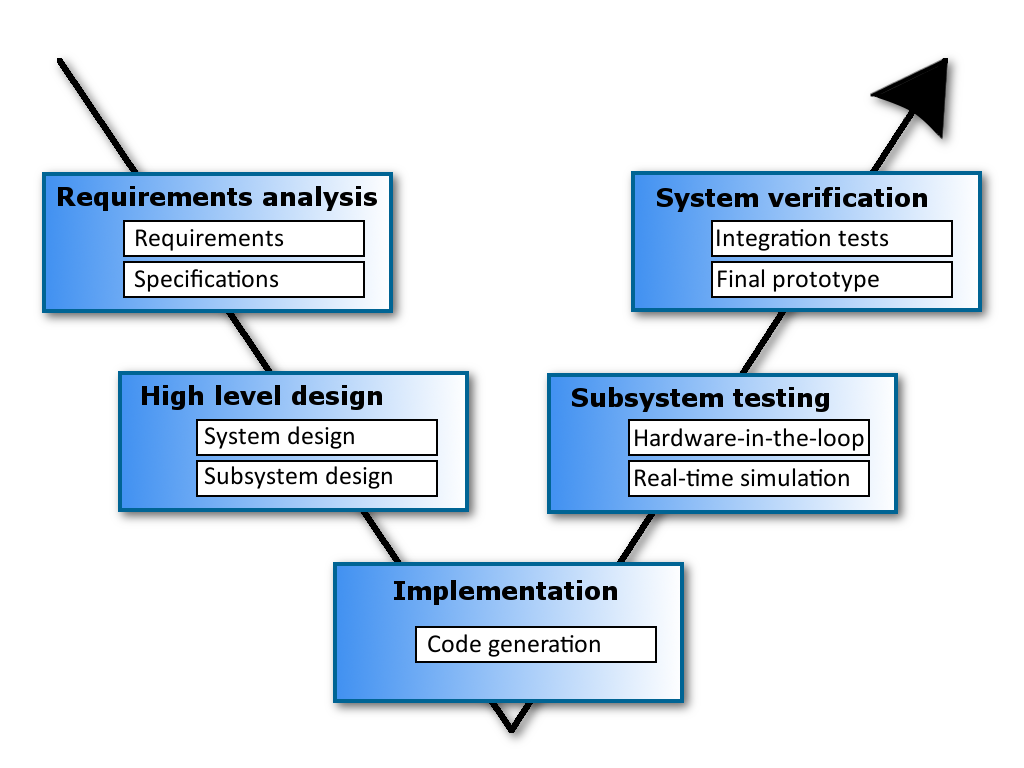
\includegraphics[scale=0.35]{pictures/model_based_design_Vcycle.png}
\caption{The V-cycle of Model-Based design process}
\label{fig:modelBasedDesignProcess}
\end{figure}

That is why a Model-Based design pattern was created and deployed in practise (see \ref{fig:modelBasedDesignProcess}). Model-Based design overcomes obstacles of the traditional design process by unification of all phases of the development cycle into one model creation tool. Whole process is centered around a mathematical model of a desired system. This method is usually shown as V shaped design process. Starting by specifications and requirements we are practically describing a mathematical model of a system and such formal specifications can be verified, tested and optimized. Following design phase then fluently shifts the model creation to another dimension, the sub-component and component representation using model design tools like Matlab/Simulink/Stateflow, Ptolemy or SystemModeler.

Testing and verification in this part of the process is non-trivial and although there exist plenty of tools and algorithms to achieve model correctness assurance (an example can be S-Taliro tools) this is still active area of research. Big advantage of such method is the possibility to real-time simulate desired system and debug the model. After all corrections, final model is used to generate the code which rapidly accelerate the whole development process. Finally when we are ready to test the model against hardware by Hardware-in-the-Loop simulation and verify the system from the integration point of view by integration tests. This pattern helps us to discover any design flaws in early stage of the development and enables us to quickly redesign the model.

\subsection{Example of a model of Cyber-Physical system}

As an example of model of a cyber-physical system can be used an experimental electro-mechanical brake model with disk wiping. [Oehlerking, “Experimental electro-mechanical brake model with disk wiping”, 2015] In their case study Strathmann and Oehlerking present a simplified model of electro-mechanical brake and three verification tools that were tested on the model. Model consists of a plant model and a controller.

\section{Model Verification and testing}

During model-based design process we gather clearer and more concrete representation of the desired system but in addition at each phase we are able to test and verify the model if by any chance our design does not contain some errors. In the first phase we are able to test requirements and specifications whether there are any contradictions, duplicities or overcomplicated expressions [TODO: confirm and support by references]. During the system and subsystem design phase we are able to simulate real-time usage of all these models and spot any indicators of an unwanted behavior. With the right approach and proper way of specification this phase already gives us possibility to verify if the model meet our safety specifications with certain robustness. Implementation phase is closely connected with semantics verification, code and resources testing. In the subsystem testing part of the process we are verifying our model structures against a real hardware realization such as testing controller against emulated hardware plant. Last stage of system verification are integration tests, creation of the first prototype and its testing in a real physical environment.

\subsection{Model checking of the system design}

Model checking is generally used technique for the verification of the properties of software and hardware systems. Commonly we represent a system properties by modal or temporal logic formulas with the Boolean valued semantics. But when we operate in an area of systems whose state space is some general metric space, the model checking problem becomes difficult and in most of the cases undecidable. [Fainekos, “Robustness of Temporal Logic Specifications for Finite State Sequences in Metric Spaces”, 2006] Models of cyber-physical systems belong exactly in this category, because general metric transition systems model the interaction between continuous physical world and some software and/or hardware system. Thus deciding the Boolean truth value of a temporal logic specification for such system can give us absolutely no conclusions about the real system. Real system does not have to always behave the same way as it was designed to behave, depending on the environment influences and actual state of a physical world, there may be a delay or randomness. For example the braking system changes its behaviour as the materials which the system consists of are changing their properties. This is a very serious safety issue, especially in an area of systems that are to be as safest and reliable as possible.

\subsection{Metric Temporal Logic/ Temporal Logic}

\section{S-Taliro tools}

\section{Our approach}

\subsection{Model of Jan Kacetl}

\section{Conclusion}

\subsection{Dummy subsection}

You may generate list of references using iso690 Bib\TeX{} style, a non-complete implementation of \cite{iso690}.

\bibliographystyle{iso690}
\bibliography{mybibliographyfile}
    
\end{document}
